\section{Отслеживание контакта в случае \textit{mecanum} колеса}

Обозначим угол наклона оси ролика к плоскости колеса $\psi$. В предыдущей конфигурации этот угол равен нулю. Расширим алгоритм отслеживания контакта, описанный выше для случая $\psi = 0$ на конфигурацию \textit{mecanum}, $\psi > 0$. В этом случае, в первую очередь, отметим отличия в геометрической форме роликов. Каждый ролик -- это твердое тело, ограниченное поверхностью вращения некоторой кривой вокруг его оси. В случае $\psi = 0$ эта кривая -- дуга окружности, но при $\psi > 0$, для того, чтобы проекция внежней границы колеса на его плоскость оставалась окружностью, форма роликов должна быть более сложной \cite{Gfrerrer2008}.

\subsection{Неявный алгоритм отслеживания контакта}

Здесь, как и всюду, будем предполагать, что плоскость колеса вертикальна во все время движения.

Введем систему отсчета $O_A{\bf i}{\bf j}{\bf k}$, жестко связанную с колесом, с началом в его центре $O_A$. Вектор ${\bf k}$ направлен вдоль оси колеса, ${\bf i}$ и ${\bf j}$ лежат в его плоскости.

Введем также две вспомогательные системы отсчета $O_A{\bf i}_1{\bf j}_1{\bf k}_1$ и $O_B{\bf i}_2{\bf j}_2{\bf k}_2$, где $O_B$ -- центр ролика.

Вектор ${\bf i}_2$ направим вдоль оси симметрии ролика, см. фиг.~\ref{ContactScheme}.
Вектор ${\bf j}_2$ ортогонален ${\bf i}_2$ и лежит в вертикальной плоскости.
Третий вектор ${\bf k}_2$ определяется естественным образом как
$$
{\bf k}_2={\bf i}_2\times {\bf j}_2.
$$
% \begin{figure}[hb]
% \centerline{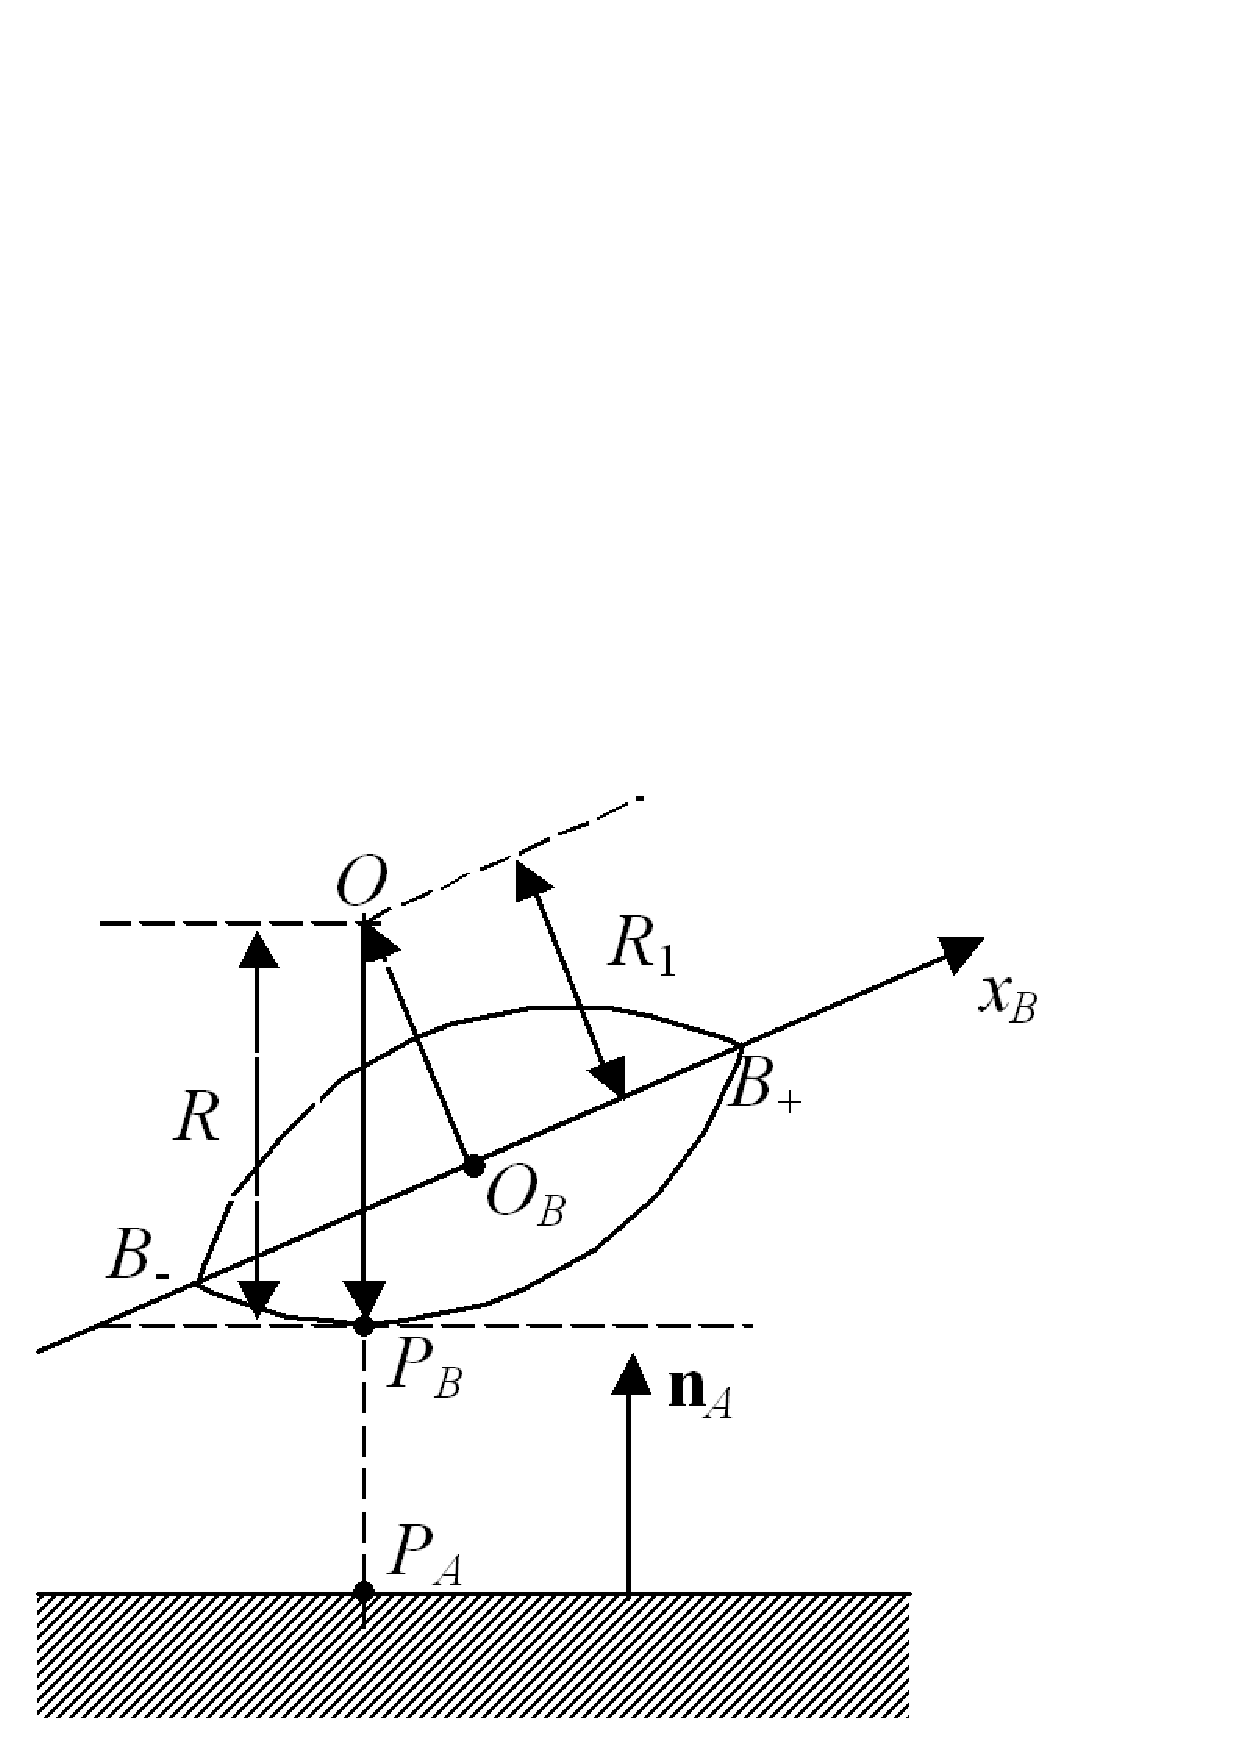
\includegraphics[bb= 0cm 0cm 20cm 17cm,scale=0.30]{RollerSection.png}}
% \caption{Contact tracking scheme.}
% \label{ContactScheme}
% \end{figure}

Во время счета компоненты всех векторов задаются относительно неподвижной системы отсчета, а положения и ориентации всех тел системы в момент времени $t\in [t_0,t_1]$ считаются известными.

Таким образом, для системы $O_B{\bf i}_2{\bf j}_2{\bf k}_2$, имеем:
$$
{\bf i}_2=T_B\cdot (1,0,0)^T,\quad\vecrho =
\left( {\bf r}_{O_A}-{\bf r}_{O_B}\right) /
\left| {\bf r}_{O_A}-{\bf r}_{O_B}\right| ,
$$
где $T_B$ -- матрица ориентации ролика, а единичный вектор $\vecrho$ направлен вдоль луча, выпущенного из центра колеса $O_A$ в сторону центра ролика $O_B$.

Вектор ${\bf i}_1$ лежит на пересечении плоскости колеса и горизонтальной плоскости.
${\bf k}_1 = {\bf k}$ ортогонален плоскости колеса и совпадает с одним из векторов базиса, связанного с колесом, и всегда горизонтален.
Тогда имеем ${\bf j}_1(t)=(0,1,0)^T$ и ${\bf i}_1(t)={\bf j}_1(t)\times {\bf k}_1(t)$.

Теперь рассмотрим соотношения, позволяющие вычислить компоненты базисных векторов векторов системы отсчета $O_B{\bf i}_2{\bf j}_2{\bf k}_2$.

Отметим, что вектор ${\bf i}_2$, направленный вдоль оси ролика, по определению не может принять вертикальное положение, если ролик находится в контакте с опорной плоскостью.
Более того, в случае \textit{mecanum} ролик повернут на постоянный угол $\psi > 0$ относительно оси $O_AO_B$, и потому во все время движения верно соотношение ${\bf i}_2\ne (0,1,0)^T$.
Таким образом, вектор ${\bf c}={\bf i}_2\times (0,1,0)^T$ также отличен от нуля.
Положим ${\bf k}_2={\bf c}/|{\bf c}|$. Теперь можно определить ${\bf j}_2$ как
${\bf j}_2={\bf k}_2\times {\bf i}_2$.

Для определения компонент вектора $\vecrho$ воспользуемся кинематическими соотношениями, условиями ортогональности векторов, следующими из определений введенных систем отсчета:
$$
\vecrho\cdot {\bf i}_2=0,\quad\vecrho\cdot {\bf k}_1=0.
$$
и их дифференциальными вариантами:
$$
\dfrac{d}{dt}\vecrho\cdot {\bf i}_2+\vecrho\cdot\dfrac{d}{dt}{\bf i}_2=0,\quad
\dfrac{d}{dt}\vecrho\cdot {\bf k}_1+\vecrho\cdot\dfrac{d}{dt}{\bf k}_1=0.
$$

Величина $c_{\beta }=\cos\beta ={\bf i}_2\cdot (0,1,0)^T$ косинуса угла $\beta $ наклона оси ролика к вертикали $(0,1,0)^T$ также играет важную роль в алгоритме отслеживания контакта.

Если текущее значение переменной величины $c_{\beta }$ меньше некоторого уровня $c_{\beta\max }$, и если одновременно расстояние от центра ролика $O_B$ до опорной плоскости меньше радиуса колеса $R$, то ролик находится в контакте с опорной плоскостью. В противном случае контакт отсутствует.

% Remark here that usually to arrange the unilateral constraint in the multibody
% system dynamics model the developer has to implement anything like hybrid 
% automata construct. In our omni wheel model on the contrary this is not the 
% case. It turned out sufficient to implement ``simple'' ``{\tt if}'' construct 
% to switch states ``contact'' and ``no contact'' for each individual roller, and
% simultaneously to advance forward ``contact'' state from one roller to its 
% neighbour. The whole picture looks like from time to time neighbouring rollers
% mutually exchange by their states.

На фиг.~\ref{ContactScheme} также легко видеть, что координаты точки $P_B$ контакта ролика и плоскости даются выражением
$$
{\bf r}_{P_B}={\bf r}_{O_B}+R_1\vecrho -R{\bf j}_1+\mu {\bf k}_1,
$$
где число $\mu$ требуется вычислить. Здесь величина $R_1$ равна расстоянию между точками $O_A$ и $O_B$.
Чтобы получить число $\mu$, умножим последнее уравнение скалярно на ${\bf k}_2$. Отсюда
$$
\mu =\left[R{\bf j}_1\cdot{\bf k}_2-R_1{\vecrho }\cdot {\bf k}_2\right] /
{\bf k}_1\cdot{\bf k}_2,
$$
поскольку ${\bf r}_{P_B}-{\bf r}_{O_B}$ лежит в вертикальном сечении осесимметричной поверхности ролика, и вектор ${\bf k}_2$ по построению ортогонален этому сечению. В результате радиус-вектор ${\bf r}_{P_B}$ точки контакта $P_B$ определяется однозначно.

\section{Явный алгоритм отслеживания контакта}

Еще одним способом вычисления компонент радиус-вектора ${\bf r}_{P_B}$ точки контакта point $P_B$ или, точнее, точки ролика, ближайшей к опорной плоскости, является применение следующего набора равенств.
Лучше всего этот способ иллюстрирует геометрическая схема на фиг.~\ref{fig:figure3}. Во-первых, имеем
$$
{\bf r}_{P_B}={\bf r}_{O_B}+\overrightarrow{CD}+\overrightarrow{DG},\quad
\overrightarrow{CD}=-m{\bf i}_2,\quad\overrightarrow{DG}=-h{\bf j}_1,
$$
где $m=R_1\sin q/\cos q/\cos\psi $, $h=R-R_1/\cos q$. Здесь $q$ -- текущее значение угла отклонения вектора ${\bf r}_{O_A}-{\bf r}_{O_B}$ от 
направления вектора $\overrightarrow{DO}$. Таким образом,
$$
\cos q=\vecrho\cdot{\bf n}_A,\quad\sin q=
\left({\bf n}_A\times\vecrho\right)\cdot {\bf k}_1.
$$
\begin{figure*}[ht]
\centerline{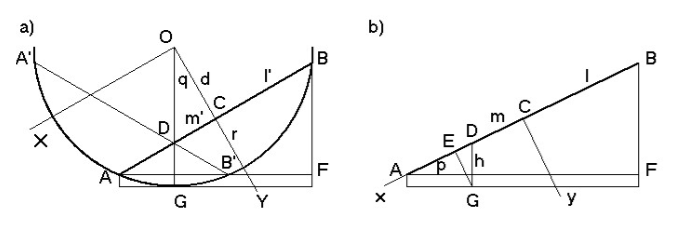
\includegraphics[scale=0.7]{content/parts/3_friction/mo2015/stepanov.png}}
\caption{Явная схема отслеживания контакта}
\label{fig:figure3}
\end{figure*}

Поясним фиг.~\ref{fig:figure3} более детально.
В части (а) приведена проекция колеса на его плоскость и соответственно, проекция ролика, находящегося в общем положении так, что его ось находится под углом к плоскости проекции.
Далее, $G$ -- точка контакта между роликом и опорной горизонтальной плоскостью в настоящий момент, $m'$ -- отрезок $DC$ проекции оси ролика на плоскость колеса. Лекго видеть, что длина этой проекции равна $m'=m\cos\psi$, поскольку ось ролика $AB$ повернута вокруг прямой $OC$ на угол $\psi$, см. вертикальное сечение, содержащее ось ролика в части (b).
Таким образом, чтобу получить точку контакта $P_B$ ($G$ на рис.), нужно пройти два отрезка прямых от центра ролика $O_B$ ($C$ на рис.): (a)~отрезок $CD$ оси ролика длины $m$; 
(b)~отрезок $DG$ вертикали длины $h$.
Как было отмечено выше, все величины требуется явно выразить через известные координаты.

Чтобы исключить <<перекрытие>> роликов, т.е. ситуацию, при которой два ролика могут находиться в контакте одновременно, более чем при одном (граничном) значении угла поворота колеса, необходимо ограничить длины роликов величиной (см. фиг.~\ref{fig:figure3})
$$
L=2R\sin\alpha / \cos\psi,
$$
и при этом их концы оказываются усечены. Подробно форма кривой, образующей поверхность роликов, описана в \cite{Gfrerrer2008}.
При такой конструкции переход колеса с одного ролика на другой происходит мгновенно.
Отметим, что при этом след колеса на плоскости имеет разрыв, поскольку точка контакта мгновенно переходит на противоположный <<борт>> колеса. Это обстоятельство, впрочем, не препятствует эффективному численному решению.

Описанные алгоритмы отслеживания контакта дают практически одинаковые результаты, относительные различия между которыми имеют порядок $10^{-8}$. Предсказуемо, явный алгоритм быстрее приблизительно в $1.5$ раза.
